\chapter{Results} In this chapter, I analyze the benchmark results and discuss
their implications for data scientists using incremental random forest
classifiers. In each trial, each incremental random forest classifier received
batches sequentially, retraining itself after every new batch. For each tested
workload, I first contrast sample training times of several incremental growth
and tree replacement strategies. Then, I analyze a range of hybrid strategies
and explore the ideal hybrid strategy for each workload based on concept drift
and batch size.

% TODO ERF


\section{Workload A: Large batches, no concept drift}

The Homesite Quote Conversion dataset is a Kaggle dataset that provides over
fifty numerical and categorical metrics on each of 200,000 customers. The
classification goal is to determine whether a potential customer will purchase
home insurance given the provided metrics about their quoted price, previous
activity, coverage information, and more. \cite{Homesite} To study how
incremental random forests would perform on workloads with large batch sizes
and no concept drift, I randomly divided the Homesite dataset into fifteen
batches of 2,000 data points each. Then, I ran tests using both deep and
shallow random forests, measuring the training time required by each sample
strategy to accommodate each new batch of data.

\begin{figure} 
  \centering 
  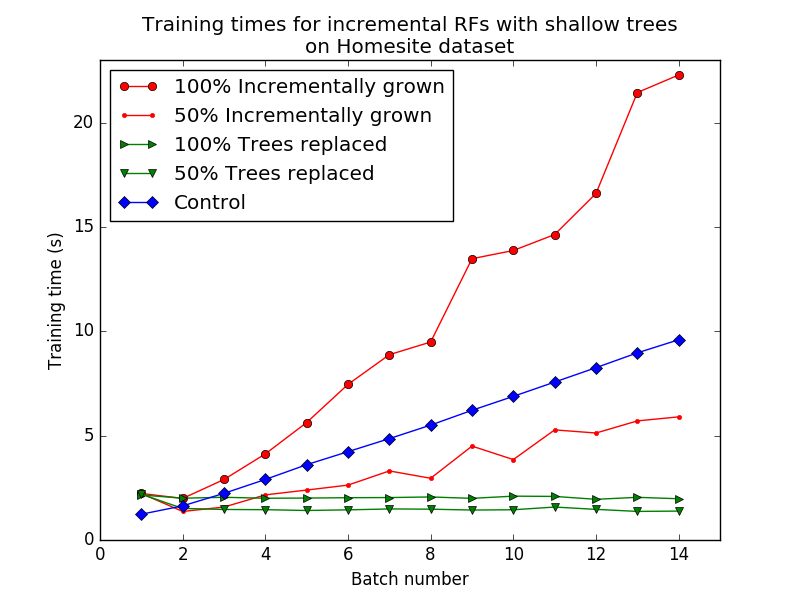
\includegraphics[width=4.0in]{g1_1}\\
  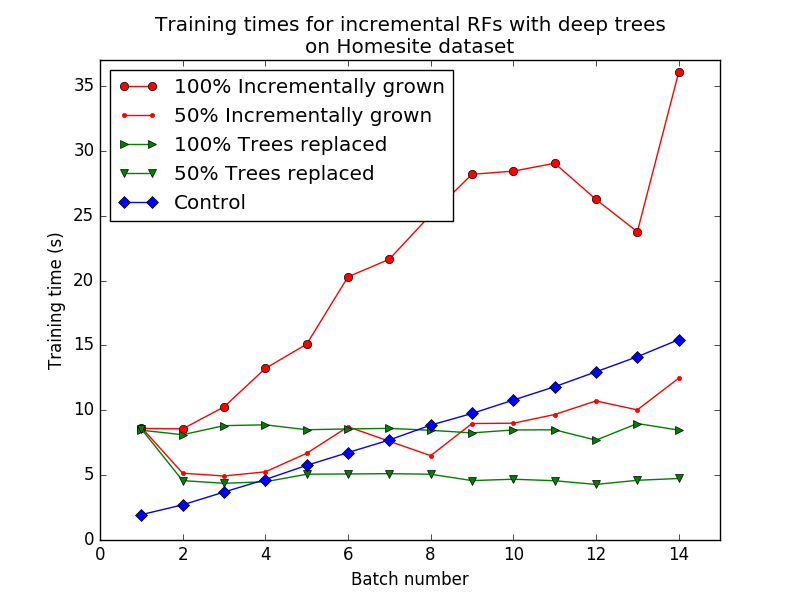
\includegraphics[width=4.0in]{g2_1} 
  \caption{These graphs show the training
  times for the incremental growth strategy, the tree replacement strategy, and
the control setting on the batched Homesite Quote Conversion dataset.}
\label{fig:homesite1} 
\end{figure}

As seen in Figure \ref{fig:homesite1}, retraining the entire tree from scratch
on all data caused the training time for the control setting to be much higher
on later batches than the training time for the experimental settings, with one
notable exception. When all trees are grown incrementally after each batch, the
training time is higher than the control. This occurs because every full added
level of nodes doubles the number of leaves in the tree. As a result, the next
incremental training step must examine twice as many leaves for potential new
splits. While Spark random forests mitigate this exponential growth by batch
processing leaves, the results still reveal the significant overhead. As a
result, my findings indicate that no more than around 50\% of trees should be
incrementally grown after every batch if training time is a primary concern.
These findings are consistent in both random forests with deep trees and those
with shallow trees.

In contrast to the incremental growth strategy and the control, the tree
replacement strategy shows similar training times across all batches. This
occurs because the system grows the same number of trees on the same quantity
of data after each timestep. While a data scientist would likely not wish to
regrow 100\% of trees, I consider the training times for a 100\% tree
replacement strategy to demonstrate the worst-case training time for a random
forest classifier using this strategy. Even when the forest is entirely regrown
on each new batch, the training time eventually drops below the monotonically
increasing control training times. As seen, the random replacement strategy
will always be more efficient than the control after a certain batch number on
workloads such as the batched Homesite Quote Conversion dataset.

\begin{figure} 
  \centering 
  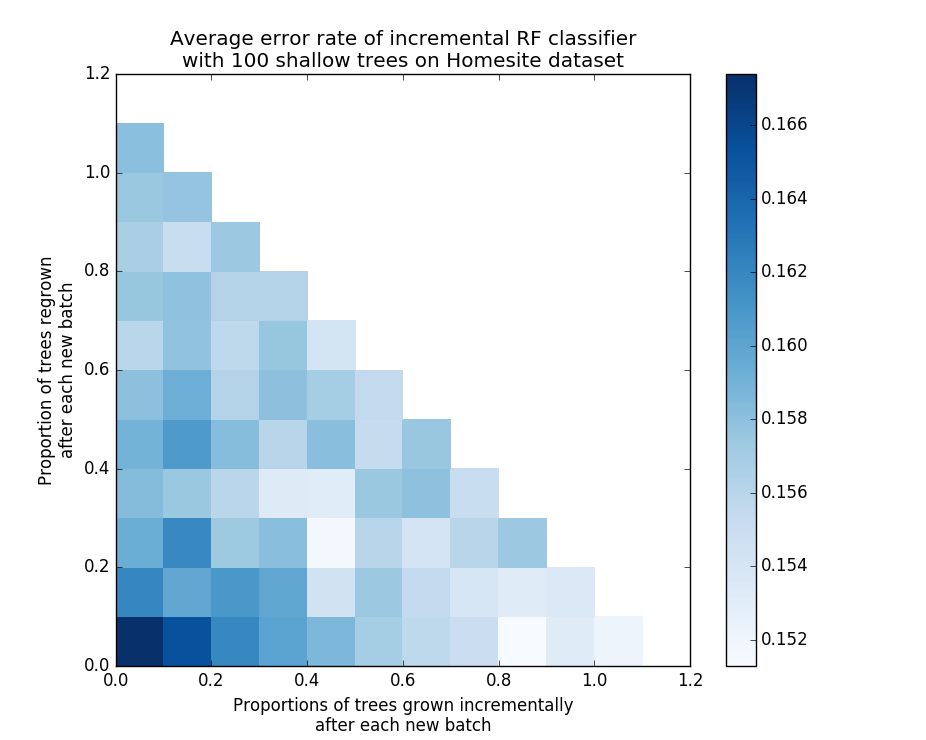
\includegraphics[width=5.0in]{homesite_shallow}
  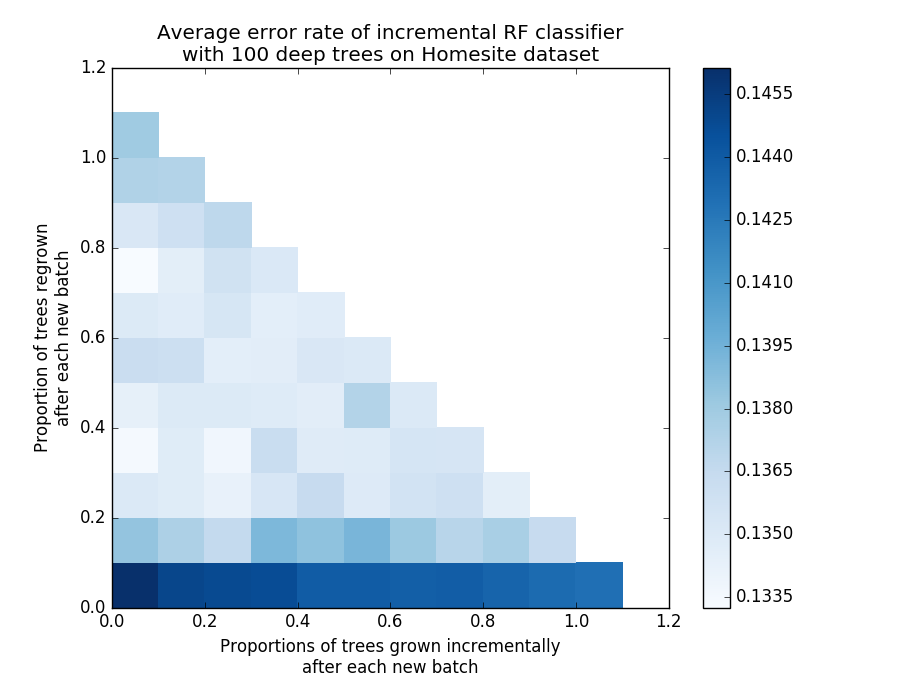
\includegraphics[width=5.0in]{homesite_deep} 
  \caption{These two plots show
    the average error rates of various hybrid tree replacement and incremental
    growth strategies on the Homesite batched dataset. The axes indicate the
percentage of trees that are modified according to each strategy.}
  \label{fig:homesitehybrid} 
\end{figure}

Figure \ref{fig:homesitehybrid} shows the results of measuring the average
predictive error rates of 50 different hybrid incremental random forests. In
random forests with shallow trees, hybrid strategies with a high proportion of
trees incrementally grown performed better than other strategies. In general,
using shallow trees should favor incremental strategies, as shallow trees are
better able adapt to new information in batches than deep trees.  Since forests
with deep trees are generally more accurate than those with shallow trees, a
data scientist would likely use shallow trees if training time was a primary
concern. Considering the training time data shown in Figure
\ref{fig:homesite1}, the optimal strategy for this setting seems to be
regrowing approximately 40\% of trees and incrementally growing another 40\%. 

In random forests with deep trees, hybrid strategies with a nonzero proportion
of trees regrown after every new batch show the lowest error rate. This trend
reveals that deep decision trees poorly accommodate additional information from
later batches. While these deep forests with purely incremental strategies have
lower error rates than shallow forests, they perform significantly worse than
all other hybrid strategies. Therefore, the optimal strategy for this setting
seems to be to regrow around 30\% of trees with each new batch. This strategy
minimizes both training time and predictive error rate.

\section{Workload B: Small batches, no concept drift}

The Otto Group Product Classification dataset contains 200,000 data points
representing products sold by the Otto Group. Each data point is characterized
by nearly 100 numerical features representing qualities of each product; the
classification task is to distinguish one particular product category, ``Class
2,'' from the others. By randomly downsampling the dataset, I segmented the
data into batched workloads of approximately 100 points per batch, much smaller
than the 2,000-point batches of the Homesite dataset. \cite{Otto} My initial
analysis, as with the Homesite dataset, involved contrasting the training times
of the two incremental random forest strategies on the data. I trained random
forest classifiers using each of two strategies on fifty 100-point batches of
the Otto dataset to demonstrate any trends over time.

\begin{figure}
  \centering
  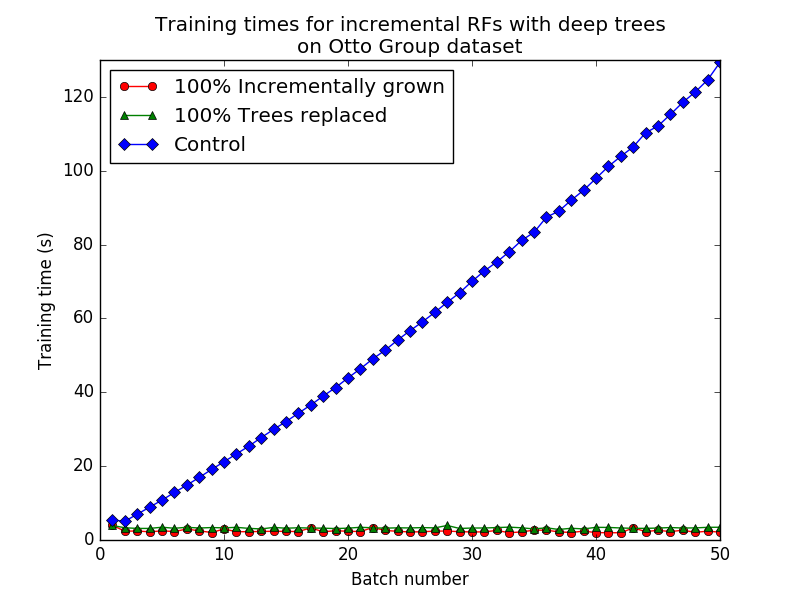
\includegraphics[width=4.0in]{otto4} \\
  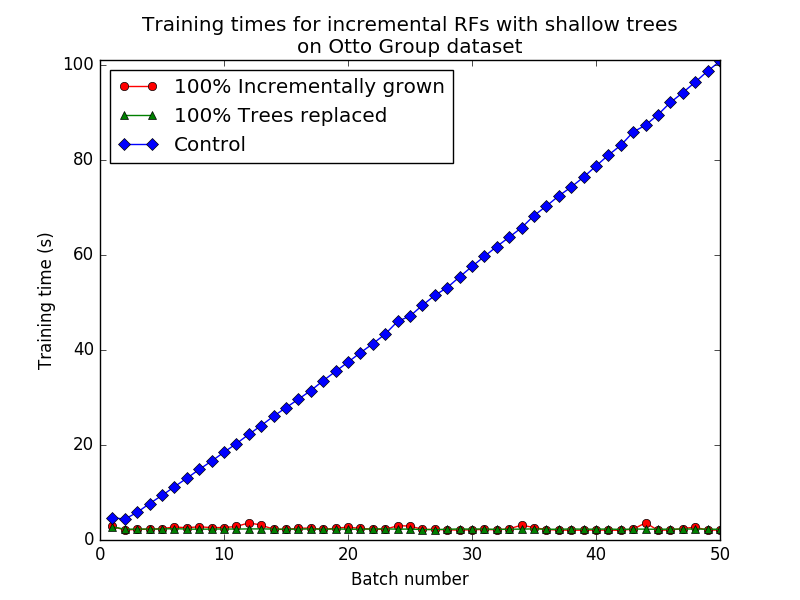
\includegraphics[width=4.0in]{otto2}
  \caption{These graphs show the error rates and training times for the
incremental growth strategy, the tree replacement strategy, and the control
setting on the batched Otto Group Product Classification dataset.}
  \label{fig:otto1}
\end{figure}

As seen in Figures \ref{fig:otto1},the control demonstrates the largest
training time after each batch, as it must be retrained from scratch on the
aggregate data. In comparison, the training times for the experimental
strategies are far smaller, even when every tree in the forest is modified
after each batch. This trend is consistent in both random forests with deep
trees and those with shallow trees. 

\begin{figure}
  \centering
  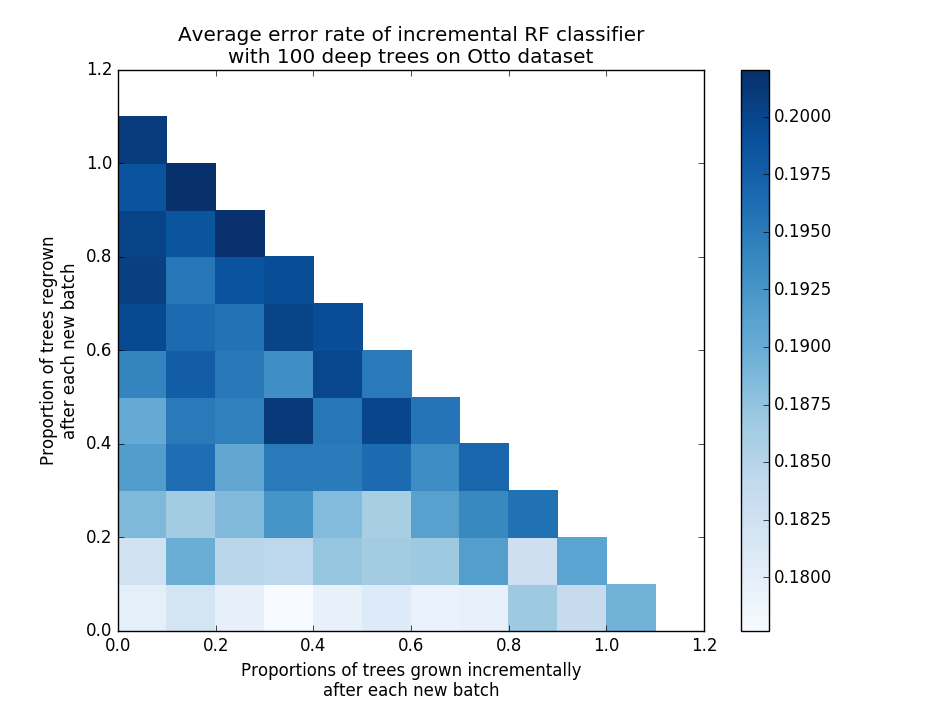
\includegraphics[width=5.0in]{otto_deep_med}\\
  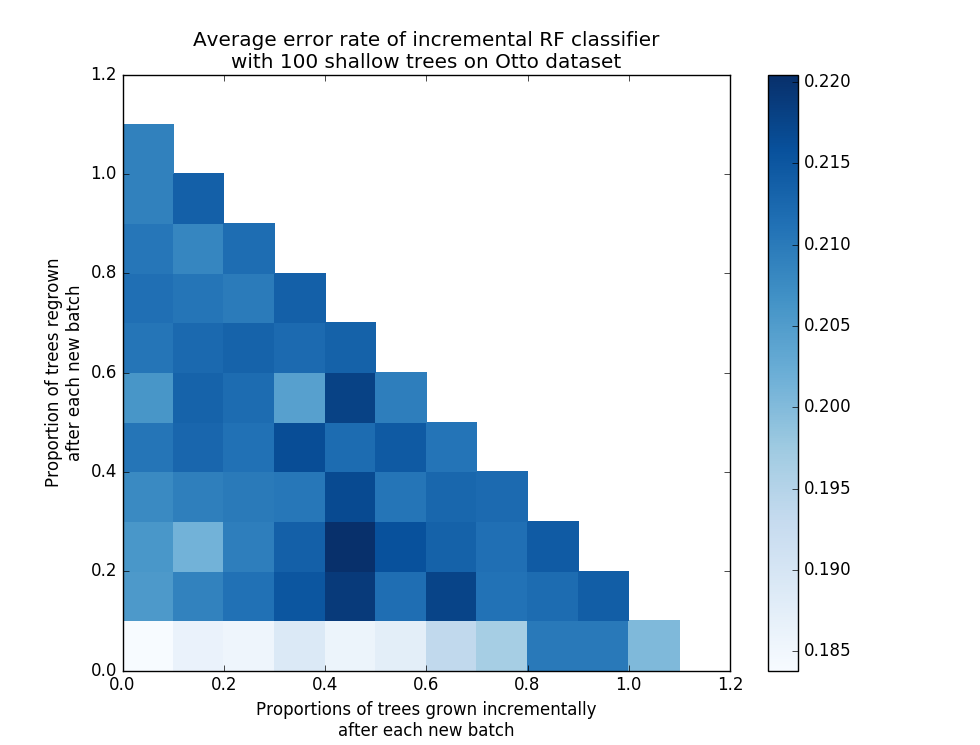
\includegraphics[width=5.0in]{otto_shallow_med}
  \caption{These two plots show the average error rates of various hybrid tree
  replacement and incremental growth strategies on the Otto Group batched
dataset. The axes indicate the percentage of trees that are modified according
to each strategy.}
  \label{fig:ottohybrid}
\end{figure}

Figure \ref{fig:ottohybrid} displays the predictive error rate of various
hybrid incremental random forest classifiers. As shown, for smaller batch sizes
such as 100, strategies that involve only incremental growth generally perform
better than strategies that incorporate some proportion of regrown trees. This
trend is present in both random forest classifiers comprised of deep trees and
those with shallow trees, though the trend is stronger among forests with
shallow trees. 

Trees grown on one batch naturally overfit to that batch. With a small batch
size, there is a higher likelihood that a batch's data distribution differs from the
overall data distribution of the full dataset. As such, tree replacement
strategies could grow trees that fit well to one batch, but that fit poorly to
the rest of the data, increasing the error rate. Incremental growth
incorporates the data from multiple batches into each tree, mitigating the
effect of overfitting to the wrong data distribution.

These results demonstrate that data scientists using incremental
random forests on workloads with small data batches should utilize a strategy
that only involves incremental growth. Figure \ref{fig:ottohybrid} indicates
that the specific proportion of trees that are incrementally grown can vary
with little impact on accuracy, so data scientists should choose a smaller
ratio to minimize training time.

\section{Workload C: Large batches, concept drift}

The US Department of Transportation Airline On-Time Statistics and Delay Causes
dataset contains information about every flight that took place in the last
decade. I used 18-months of this dataset, beginning in January 2014, for my
analysis. Because the distribution of airline delay data varies seasonally,
this dataset exhibits concept drift. Each month of data translated to a
10,000-point batch in an 18-batch data workload. \cite{Plane}

\begin{figure}
  \centering
  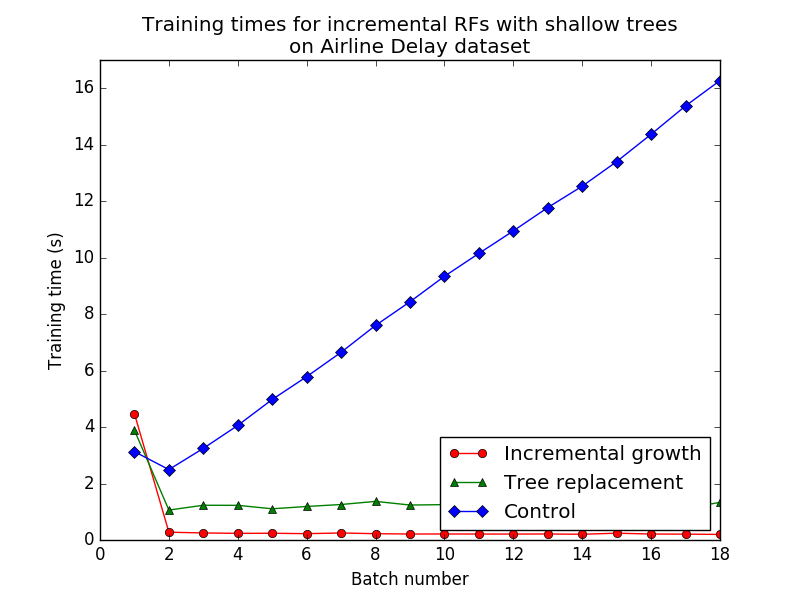
\includegraphics[width=4in]{planeshallow_line_time}
  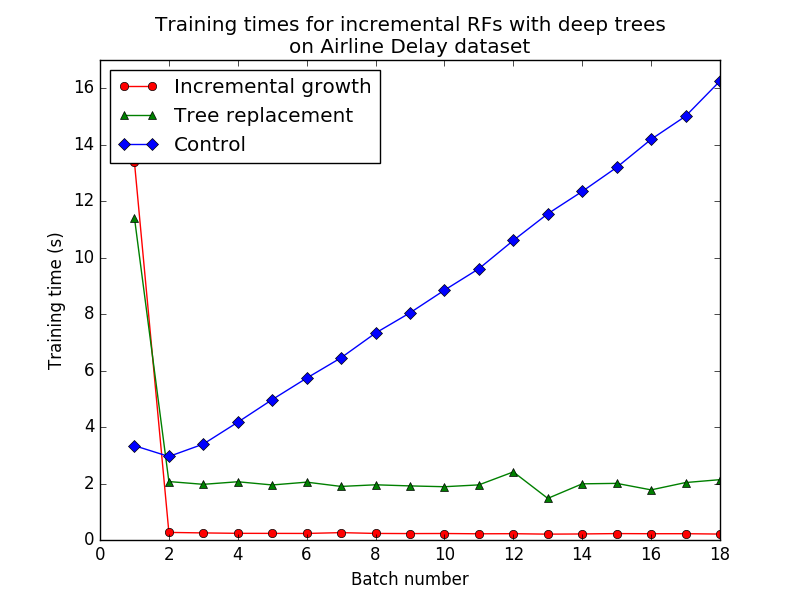
\includegraphics[width=4in]{planedeep_line_time}
  \caption{These graphs show the error rates and training times for the
incremental growth strategy, the tree replacement strategy, and the control
setting on the batched Airline Delay dataset.}
  \label{fig:plane1}
\end{figure}

In Figure \ref{fig:plane1}, I contrast the training times of several
incremental random forest classifiers using a variety of pure strategies. In
the first graph, I show the training times for the classifiers incrementally
growing 50\% and 40\% of trees, as all training time progressions for
classifiers incrementally growing a higher percentage rapidly increase to a
time significantly larger than the control. If the percentage of trees
incrementally grown is 40\% or lower, the classifier shows a lesser training
time than the control.

\begin{figure}
  \centering
  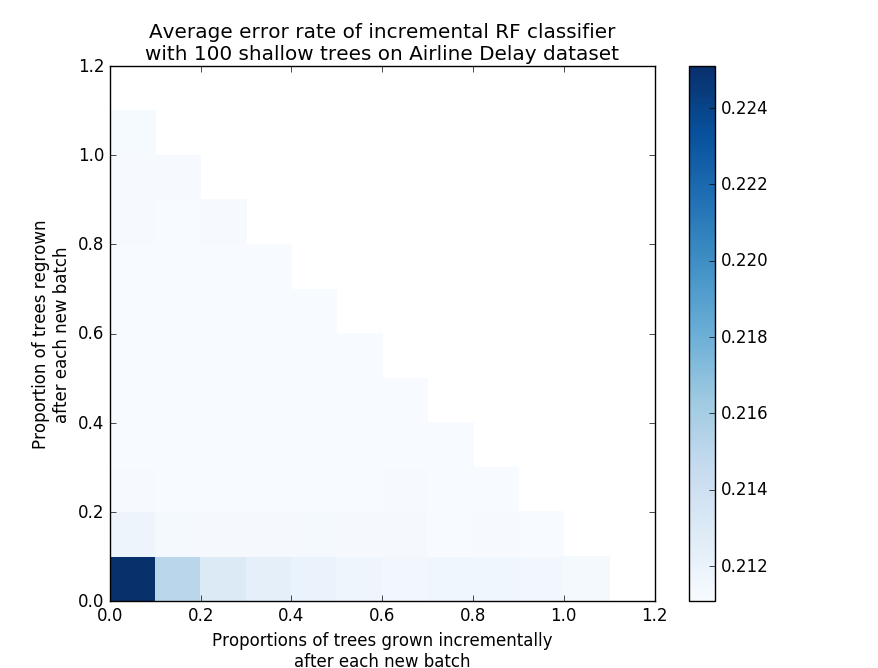
\includegraphics[width=5in]{planeshallow}
  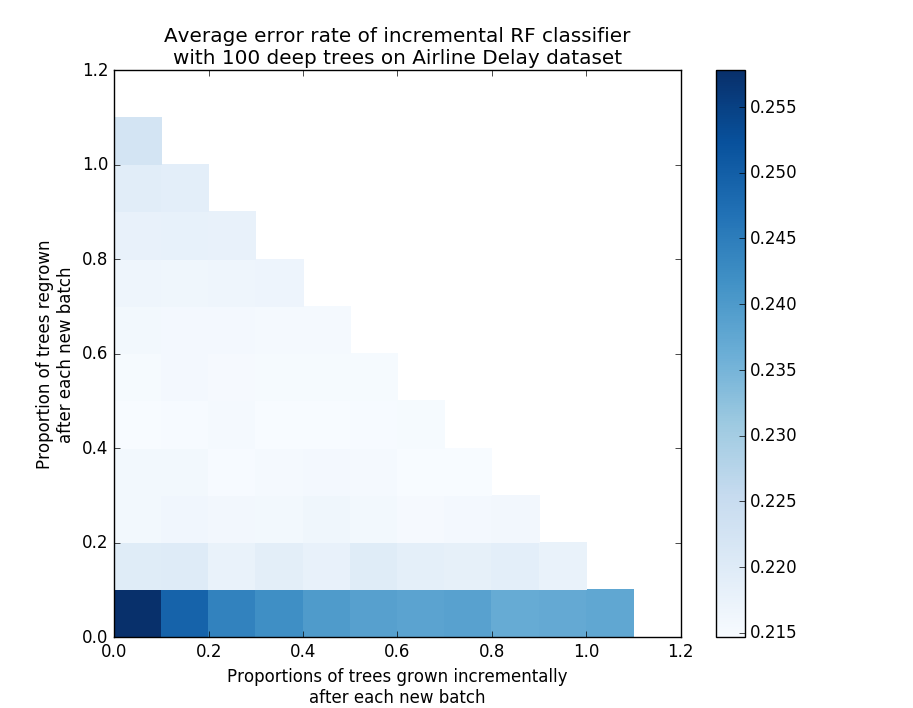
\includegraphics[width=5in]{planedeep}
  \caption{These two plots show the average error rates of various hybrid tree
  replacement and incremental growth strategies on the Airline Delay batched
dataset. The axes indicate the percentage of trees that are modified according
to each strategy.}
  \label{fig:planehybrid}
\end{figure}
 
The classifier performance results from the Homesite dataset are similar these
Airline Delay dataset results. In both, incrementally growing every tree in the
random forest quickly becomes inefficient compared to the control. The effect
is augmented when the dataset has concept drift, since more leaves will likely
be split to accommodate the shifts in data distribution. As such, data
scientists using batched incremental random forests on data workloads with a
large batch size should not incrementally grow a large proportion of trees if
efficiency is a major concern. 

Figure \ref{fig:planehybrid} demonstrates a distinct trend---incremental random
forest classifiers applied to workloads with large batch sizes and concept
drift perform far more poorly when using a purely incremental strategy than
when using any other strategy. This trend is more pronounced in forests with
deep trees. Again, the results show that deep trees have a harder time adapting
to shifts in data distribution than shallow trees. In a dataset with concept
drift, such as the Airline Delay dataset, this ability to adapt becomes a
larger factor in classification accuracy. The effect is mitigated in shallow
trees when a percentage of trees greater than 20\% is grown incrementally after
every batch.

The results in Figure \ref{fig:plane1} and \ref{fig:planehybrid} indicate that data
scientists using incremental random forest classifiers on workloads with large
batches and concept drift should regrow around 20\% of the trees in the forest
after each batch. This strategy minimizes predictive error while also
maintaining a low incremental training time.


\section{Workload D: Small batches, concept drift}

\begin{figure}
  \centering
  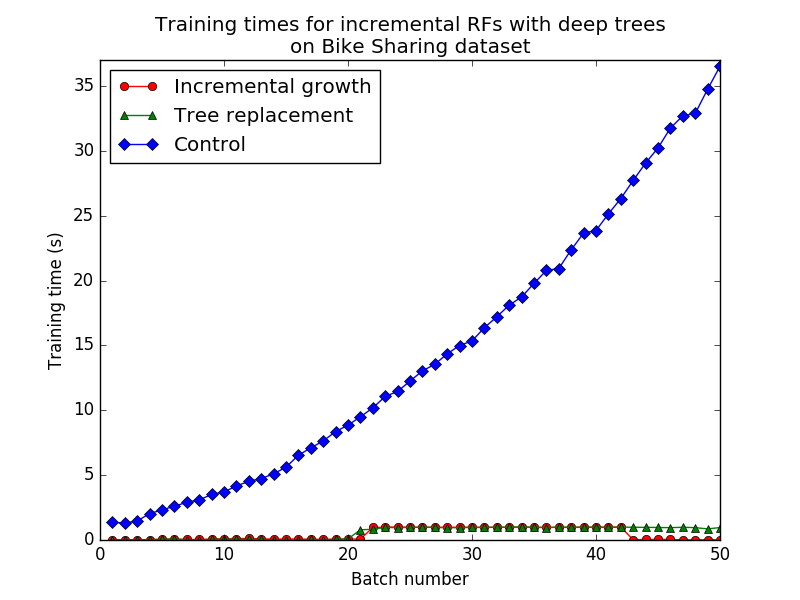
\includegraphics[width=4.0in]{deep_bikeshare_time}\\
  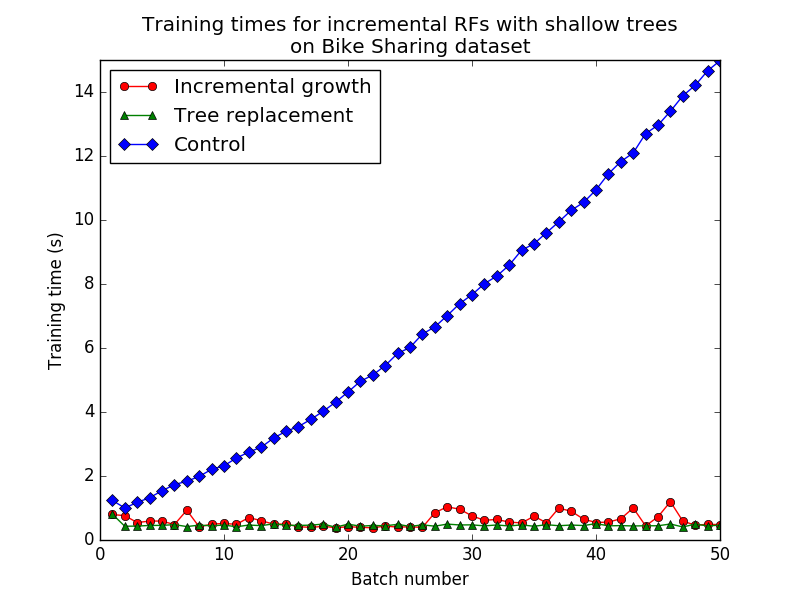
\includegraphics[width=4.0in]{shallow_bikeshare_time}
  \caption{These graphs show the training times for the
  incremental growth strategy, the tree replacement strategy, and the control
setting on the batched Homesite Quote Conversion dataset.}
  \label{fig:bikeshare1}
\end{figure}

\begin{figure}
  \centering
  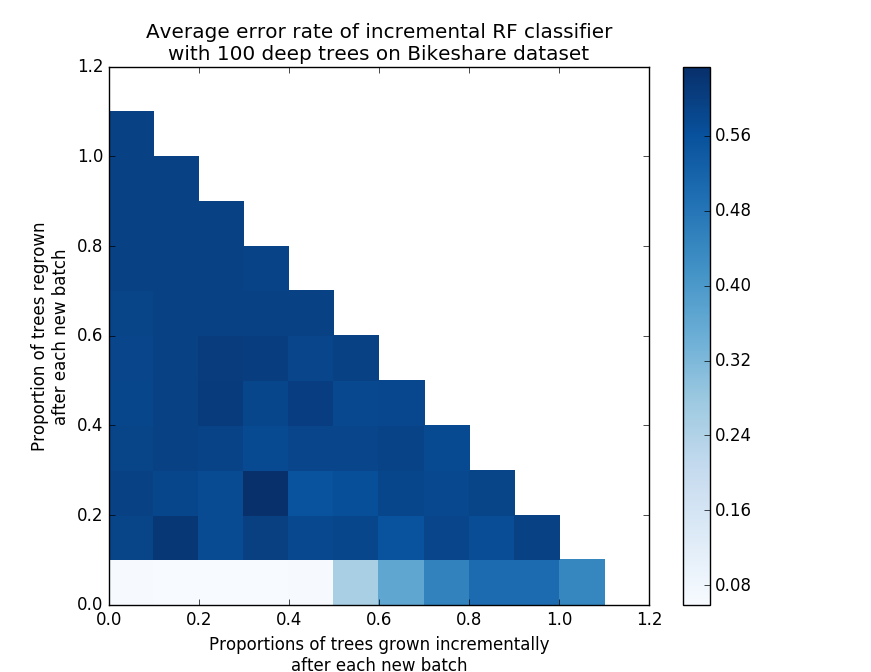
\includegraphics[width=5in]{bikesharedeep}
  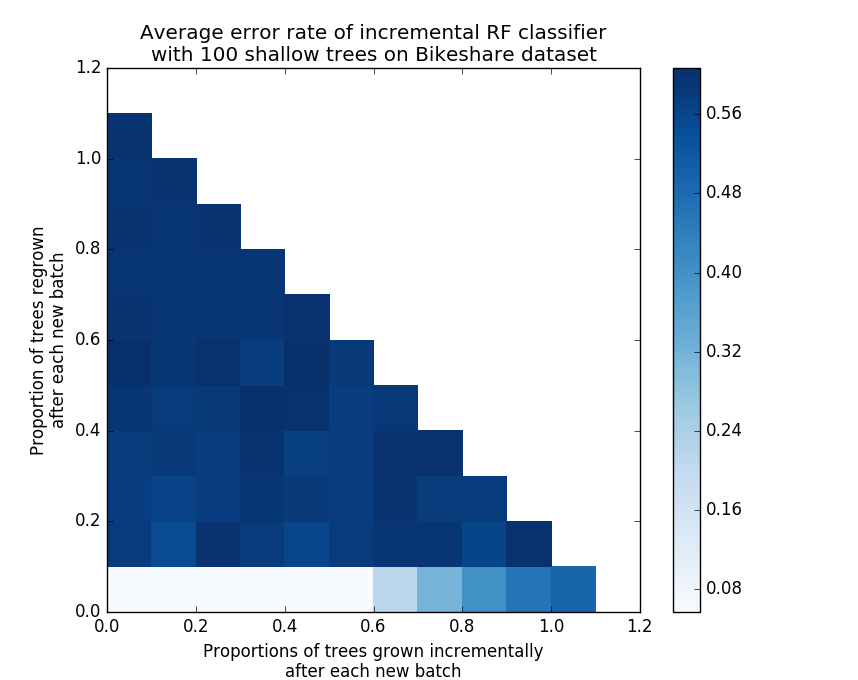
\includegraphics[width=5in]{bikeshareshallow}
  \caption{These two plots show the average error rates of various hybrid tree
  replacement and incremental growth strategies on the Bike Sharing batched
dataset. The axes indicate the percentage of trees that are modified according
to each strategy.}
  \label{fig:bikesharehybrid}
\end{figure}

The UCI Bike Sharing Dataset captures the number of rental bikes used hourly in
the Capital bikeshare system over two years. The dataset provides general
information about the temperature, weather, and other aspects of a particular
day; the classification task is whether the number of used rental bikes exceeds
120 in a given hour. Over the course of a year, the data distribution of the
Bike Sharing dataset shifts due to seasonal changes; fewer individuals
generally ride bikes in the winter, whereas the summer sees a significant spike
in rentals. \cite{Bikeshare}

Figure \ref{fig:bikeshare1} shows that the training time for the control
increases dramatically as it accumulates tens of batches. These results are
similar to the results from the Otto Group dataset, showing that when the batch
size is small, incremental strategies allow random forest classifiers to
register and adapt to new data far more quickly than ordinary random forests.
Therefore, if time is a primary concern, incremental random forests become more
desirable when the batch size of a workload is small.

Figure \ref{fig:bikesharehybrid} demonstrates that pure incremental growth
strategies are far more accurate than any other strategy on this workload. The
bikeshare dataset exhibits extreme concept shift; very few individuals rent
bikes in the middle of winter, whereas the number of rentals over the summer
nearly always passes the threshold of 120. However, since the dataset is
cyclical, a classifier that shifts too signficantly to fit, for example, the
summer trend will perform very poorly on data batches from the subsequent
winter months. The results reveal this trend is consistent in both incremental
random forests with deep trees and those with shallow trees. As a result, data
scientists should use a pure incremental growth strategy when using incremental
random forests on a data workload with small batches and large concept drift.


